Das erste automatisch erstellte Projekt enthält sechs leere Spuren und trägt den Namen \emph{Untitled}. Als erstes wollen wir eine Audiodatei importieren. Dazu benötigen wir eine oder mehrere Audiodateien, entweder im unkomprimierten Wave-Format, oder in den komprimierten Formaten MP3, Ogg Vorbis, Flac oder WavPack. Die Dateien können irgendwo auf der Festplatte liegen, oder können, falls man alle zum Projekt gehörenden Dateien beisammen haben will, nach ,,Untitled/audisources'' kopiert werden. Zurück in Traverso drückt die Taste I auf einer leeren Spur, und navigiert im sich öffnenden Dateidialog zu einer der Audiodateien. Öffnet ihr diese, wird sie in die leere Spur importiert. Die Berechnung der Wellenform dauert beim ersten Mal einige Sekunden, ab dem zweiten Mal erfolg die Darstellung ohne Verzögerung.

Um die Spur abzuspielen drückt die Leertaste. Das VUMeter zeigt dann das Ausgangssignal an. Ist das VUMeter nicht sichtbar, kann es über ``Ansicht $\rightarrow$ VUMeters'' geöffnet werden. Um den Audioclip stummzuschalten, haltet den Mauszeiger darüber und drückt die Taste U. Gemä"s unserer Notation schreiben wir diesen Befehl als \sact{U}. Eine Farbänderung zeigt an, dass der Audioclip stumm geschaltet wurde. Befindet sich der Mauszeiger während der \sact{U}-Aktion über einem leeren Bereich der Spur oder über dem Trackpanel, so wird die ganze Spur stummgeschaltet, was durch das Aufleuchten des ,,Mute''-Knopfes angezeigt wird. Erneutes drücken von \sact{U} hebt die Stummschaltung auf.

Um den Clip in zwei Teile zu schneiden, plazieren wir den Mauszeiger an der gewünschten Stelle und drücken \sact{X} -- schon haben wir zwei Clips. Um die Aktion rückgängig zu machen, drückt den Rückgängig-Knopf in der Menuleiste. Die beiden Clip-Teile werden wieder verschmelzen.

Die Lautstärke einer Spur oder eines Clips wird wie folgt geändert: Haltet den Mauszeiger auf den Clip, drückt G und haltet die Taste gedrückt. Der Mauszeiger ändert sein Symbol (\FigB\ \ref{fig_gaincursor}), und wenn ihr nun die Maus rauf und runter bewegt, ändert sich die Lautstärke. Die Notation für eine Halte-Aktion ist \hact{H}. Sobald die Taste losgelassen wird, kehrt der Mauszeiger zu seinem ursprünglichen Symbol zurück und der neue Volumenwert wird übernommen. Zeigt der Mauszeiger beim drücken der Taste auf den Hintergrund der Spur, wird die Lautstärke der ganzen Spur geändert. Ist die ganze Spur von Audioclips verdeckt, kann man den Mauszeiger stattdessen auch auf dem Trackpanel (dort wo der ,,Solo'', ,,Mute'', und ,,Rec''-Knopf sich befinden) platzieren um die Lautstärke der ganzen Spur zu ändern. Anstatt die Maus zu bewegen, kann der Wert auch mit dem Scroll-Rad geändert werden. Diese Aktionen können alle rückgängig gemacht werden und können auch direkt im History-Fenster angesprungen werden.

\begin{figure}
 \centering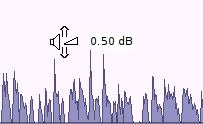
\includegraphics[width=0.4\textwidth]{images/gain-cursor.png}
 \caption{Der Mauszeiger ändert sein Symbol während einer \hact{G} Aktion.}
 \label{fig_gaincursor}
\end{figure}

Bis jetzt haben wir nur einfache Aktionen verwendet, aber es gibt natürlich noch unzählige mehr. Aber wo kann man die Aktionen nachschlagen? Glücklicherweise gibt es ein Kontextmenü, das entweder mit der rechten Maustaste oder der Aktion \sact{Q}  aufgerufen werden kann. Das Menü zeigt alle verfügbaren Aktionen und beschreibt, wie man sie ausführt (\FigB\ \ref{fig_clipmenu}).

\begin{figure}
 \centering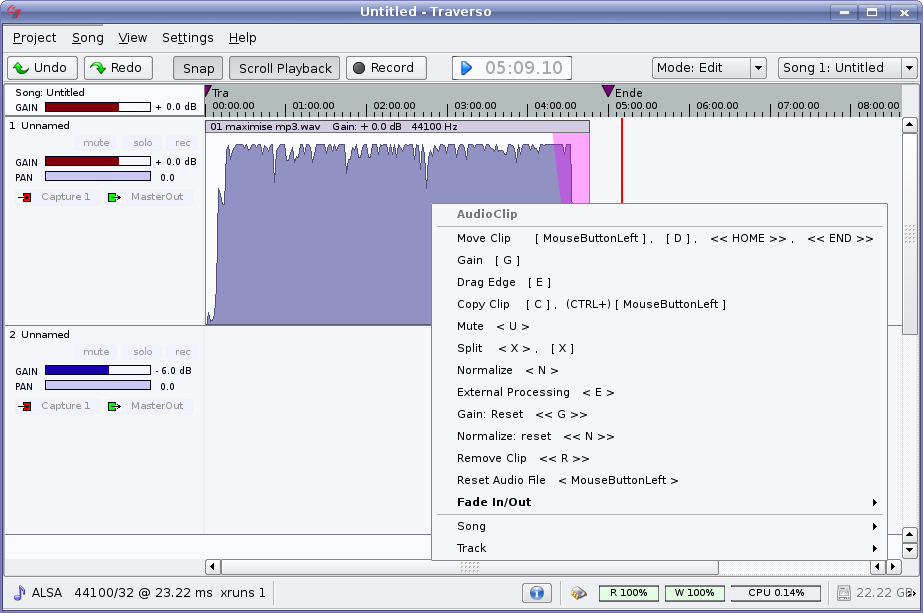
\includegraphics[width=\textwidth]{images/clipmenu.png}
 \caption{Drückt man \sact{Q} oder die rechte Maustaste, öffnet sich ein Menü mit allen verfügbaren Aktionen.}
 \label{fig_clipmenu}
\end{figure}

Audioclips können entweder mit der linken Maustaste verschoben werden, oder durch drücken von D. Gemä"s unserer Notation hei"sen die Aktionen \hact{D}, \hact{Linke Maustaste}, oder \hact{LMB}. Der Audioclip kann frei platziert werden. Sobald der Rand des Fensters erreicht wird, verschiebt sich der angezeigte Ausschnitt, wodurch auch Bereiche au"serhalb des angezeigten Ausschnittes zugänglich gemacht werden. Probiert auch die Aktionen \hact{S} und \hact{Z} um den Ausschnitt zu vergrö"sern / verkleinern oder zu verschieben.

Bis jetzt kennen wir zwei Arten von Aktionen: Die Eintasten-Aktionen \sact{K} und die Halteaktionen \hact{K}. Wir haben auch gelernt, dass Aktionen immer auf das Objekt unterhalb des Mauszeigers wirken. Bevor ihr loslegt und Traverso auf eigene Faust erkundet, lasst uns noch ein paar weitere Aktionen anschauen.

Um die Lautstärke auf den Wert 0~dB zurückzusetzen, haltet den Mauszeiger auf das entsprechende Objekt, und drückt die G-Taste zweimal schnell nacheinander. Solch einen Doppelklick notieren wir als \dact{G}. Durch mehrfaches Drücken wechselt der Volumen-Wert zwischen $-6$ und 0~dB.
